\documentclass[tikz,border=8pt]{standalone}
\usepackage{tikz}
\usetikzlibrary{calc,positioning,arrows.meta}
\usepackage[T1]{fontenc}
\usepackage[utf8]{inputenc}
\usepackage{amsmath}
%% Paleta
\definecolor{CU}{RGB}{27,38,49}
\definecolor{CNU}{RGB}{238,241,245}
\definecolor{CBRD}{RGB}{200,205,208}
\definecolor{CNEW}{RGB}{192,57,43}
\definecolor{CMO}{RGB}{36,113,163}
\definecolor{CCTR}{RGB}{211,84,0}
\definecolor{CHIT}{RGB}{29,106,57}
\definecolor{CFAL}{RGB}{183,119,13}
\definecolor{CMIS}{RGB}{21,67,96}
\definecolor{CPU}{RGB}{113,125,126}
\begin{document}

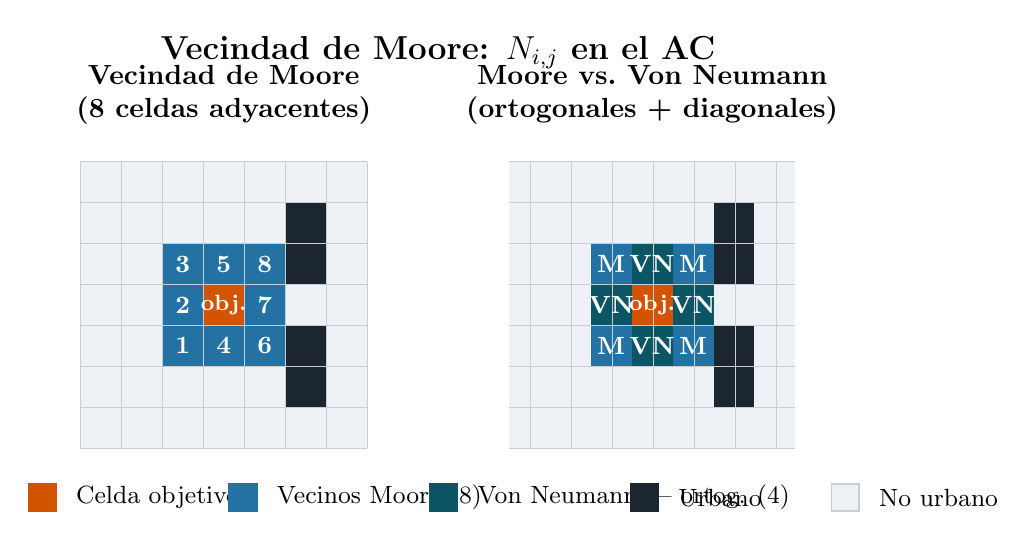
\begin{tikzpicture}[font=\sffamily]
  \fill[CNU] (0.0000cm,0.0000cm) rectangle (3.6400cm,3.6400cm);
  \fill[CU] (2.6000cm,2.6000cm) rectangle (3.1200cm,3.1200cm);
  \fill[CU] (2.0800cm,2.0800cm) rectangle (2.6000cm,2.6000cm);
  \fill[CU] (2.6000cm,2.0800cm) rectangle (3.1200cm,2.6000cm);
  \fill[CU] (2.0800cm,1.5600cm) rectangle (2.6000cm,2.0800cm);
  \fill[CU] (2.0800cm,1.0400cm) rectangle (2.6000cm,1.5600cm);
  \fill[CU] (2.6000cm,1.0400cm) rectangle (3.1200cm,1.5600cm);
  \fill[CU] (2.6000cm,0.5200cm) rectangle (3.1200cm,1.0400cm);
  \fill[CCTR] (1.5600cm,1.5600cm) rectangle (2.0800cm,2.0800cm);
  \fill[CMO] (1.0400cm,1.0400cm) rectangle (1.5600cm,1.5600cm);
  \fill[CMO] (1.0400cm,1.5600cm) rectangle (1.5600cm,2.0800cm);
  \fill[CMO] (1.0400cm,2.0800cm) rectangle (1.5600cm,2.6000cm);
  \fill[CMO] (1.5600cm,1.0400cm) rectangle (2.0800cm,1.5600cm);
  \fill[CMO] (1.5600cm,2.0800cm) rectangle (2.0800cm,2.6000cm);
  \fill[CMO] (2.0800cm,1.0400cm) rectangle (2.6000cm,1.5600cm);
  \fill[CMO] (2.0800cm,1.5600cm) rectangle (2.6000cm,2.0800cm);
  \fill[CMO] (2.0800cm,2.0800cm) rectangle (2.6000cm,2.6000cm);
  \draw[CBRD,line width=0.35pt,xstep=0.5200cm,ystep=0.5200cm] (0.0000cm,0.0000cm) grid (3.6400cm,3.6400cm);
  \node[font=\small\bfseries,text=white] at (1.8200cm,1.8200cm) {\footnotesize\bfseries obj.};
  \node[font=\small\bfseries,text=white] at (1.3000cm,1.3000cm) {1};
  \node[font=\small\bfseries,text=white] at (1.3000cm,1.8200cm) {2};
  \node[font=\small\bfseries,text=white] at (1.3000cm,2.3400cm) {3};
  \node[font=\small\bfseries,text=white] at (1.8200cm,1.3000cm) {4};
  \node[font=\small\bfseries,text=white] at (1.8200cm,2.3400cm) {5};
  \node[font=\small\bfseries,text=white] at (2.3400cm,1.3000cm) {6};
  \node[font=\small\bfseries,text=white] at (2.3400cm,1.8200cm) {7};
  \node[font=\small\bfseries,text=white] at (2.3400cm,2.3400cm) {8};
  \node[font=\normalsize\bfseries,anchor=south,align=center] at (1.8200cm,3.9900cm) {Vecindad de Moore\\(8 celdas adyacentes)};
  \fill[CNU] (5.4400cm,0.0000cm) rectangle (9.0800cm,3.6400cm);
  \fill[CU] (8.0400cm,2.6000cm) rectangle (8.5600cm,3.1200cm);
  \fill[CU] (7.5200cm,2.0800cm) rectangle (8.0400cm,2.6000cm);
  \fill[CU] (8.0400cm,2.0800cm) rectangle (8.5600cm,2.6000cm);
  \fill[CU] (7.5200cm,1.5600cm) rectangle (8.0400cm,2.0800cm);
  \fill[CU] (7.5200cm,1.0400cm) rectangle (8.0400cm,1.5600cm);
  \fill[CU] (8.0400cm,1.0400cm) rectangle (8.5600cm,1.5600cm);
  \fill[CU] (8.0400cm,0.5200cm) rectangle (8.5600cm,1.0400cm);
  \fill[CCTR] (7.0000cm,1.5600cm) rectangle (7.5200cm,2.0800cm);
  \fill[CMO!50!black!60!teal] (6.4800cm,1.5600cm) rectangle (7.0000cm,2.0800cm);
  \fill[CMO!50!black!60!teal] (7.0000cm,1.0400cm) rectangle (7.5200cm,1.5600cm);
  \fill[CMO!50!black!60!teal] (7.0000cm,2.0800cm) rectangle (7.5200cm,2.6000cm);
  \fill[CMO!50!black!60!teal] (7.5200cm,1.5600cm) rectangle (8.0400cm,2.0800cm);
  \fill[CMO] (7.5200cm,2.0800cm) rectangle (8.0400cm,2.6000cm);
  \fill[CMO] (6.4800cm,2.0800cm) rectangle (7.0000cm,2.6000cm);
  \fill[CMO] (7.5200cm,1.0400cm) rectangle (8.0400cm,1.5600cm);
  \fill[CMO] (6.4800cm,1.0400cm) rectangle (7.0000cm,1.5600cm);
  \draw[CBRD,line width=0.35pt,xstep=0.5200cm,ystep=0.5200cm] (5.4400cm,0.0000cm) grid (9.0800cm,3.6400cm);
  \node[font=\small\bfseries,text=white] at (7.2600cm,1.8200cm) {\footnotesize\bfseries obj.};
  \node[font=\small\bfseries,text=white] at (6.7400cm,1.8200cm) {VN};
  \node[font=\small\bfseries,text=white] at (7.2600cm,1.3000cm) {VN};
  \node[font=\small\bfseries,text=white] at (7.2600cm,2.3400cm) {VN};
  \node[font=\small\bfseries,text=white] at (7.7800cm,1.8200cm) {VN};
  \node[font=\small\bfseries,text=white] at (7.7800cm,2.3400cm) {M};
  \node[font=\small\bfseries,text=white] at (6.7400cm,2.3400cm) {M};
  \node[font=\small\bfseries,text=white] at (7.7800cm,1.3000cm) {M};
  \node[font=\small\bfseries,text=white] at (6.7400cm,1.3000cm) {M};
  \node[font=\normalsize\bfseries,anchor=south,align=center] at (7.2600cm,3.9900cm) {Moore vs.\ Von~Neumann\\(ortogonales + diagonales)};
  \node[font=\large\bfseries,anchor=south] at (4.5400cm,4.6900cm) {Vecindad de Moore: $N_{i,j}$ en el AC};
  \fill[CCTR] (-0.6600cm,-0.8000cm) rectangle (-0.3100cm,-0.4500cm);
  \draw[CCTR,line width=0.6pt] (-0.6600cm,-0.8000cm) rectangle (-0.3100cm,-0.4500cm);
  \node[font=\small,anchor=west] at (-0.1800cm,-0.6250cm) {Celda objetivo};
  \fill[CMO] (1.8900cm,-0.8000cm) rectangle (2.2400cm,-0.4500cm);
  \draw[CMO,line width=0.6pt] (1.8900cm,-0.8000cm) rectangle (2.2400cm,-0.4500cm);
  \node[font=\small,anchor=west] at (2.3700cm,-0.6250cm) {Vecinos Moore (8)};
  \fill[CMO!50!black!60!teal] (4.4400cm,-0.8000cm) rectangle (4.7900cm,-0.4500cm);
  \draw[CMO!50!black!60!teal,line width=0.6pt] (4.4400cm,-0.8000cm) rectangle (4.7900cm,-0.4500cm);
  \node[font=\small,anchor=west] at (4.9200cm,-0.6250cm) {Von Neumann — ortog. (4)};
  \fill[CU] (6.9900cm,-0.8000cm) rectangle (7.3400cm,-0.4500cm);
  \draw[CU,line width=0.6pt] (6.9900cm,-0.8000cm) rectangle (7.3400cm,-0.4500cm);
  \node[font=\small,anchor=west] at (7.4700cm,-0.6250cm) {Urbano};
  \fill[CNU] (9.5400cm,-0.8000cm) rectangle (9.8900cm,-0.4500cm);
  \draw[CBRD,line width=0.6pt] (9.5400cm,-0.8000cm) rectangle (9.8900cm,-0.4500cm);
  \node[font=\small,anchor=west] at (10.0200cm,-0.6250cm) {No urbano};
\end{tikzpicture}
\end{document}
